\documentclass[../AnalysisNoteJBuxton.tex]{subfiles}
\begin{document}

\subsection{Non-Flat Background}
\label{NonFlatBackground}

We observe a significant non-femtoscopic, non-flat, background in all of our correlations at large $k^{*}$.  This background increases with decreasing centrality, is the same amongst all \LamKpm pairs, and is more pronounced in the \LamKs system, as can be seen in Fig. \ref{fig:CompareAllBgds}.  

It is important to note that the difference in \LamKpm and \LamKs backgrounds is due mainly to the difference in kinematic cuts, not due to any interesting physics.  In simulation, which do a very good job of matching the experimental data, when restrictions are imposed on the $p_{\textrm{T}}$ of the \Ks to more closely match the \Kpm cuts, the backgrounds align.

\begin{figure}[h]
  \centering
  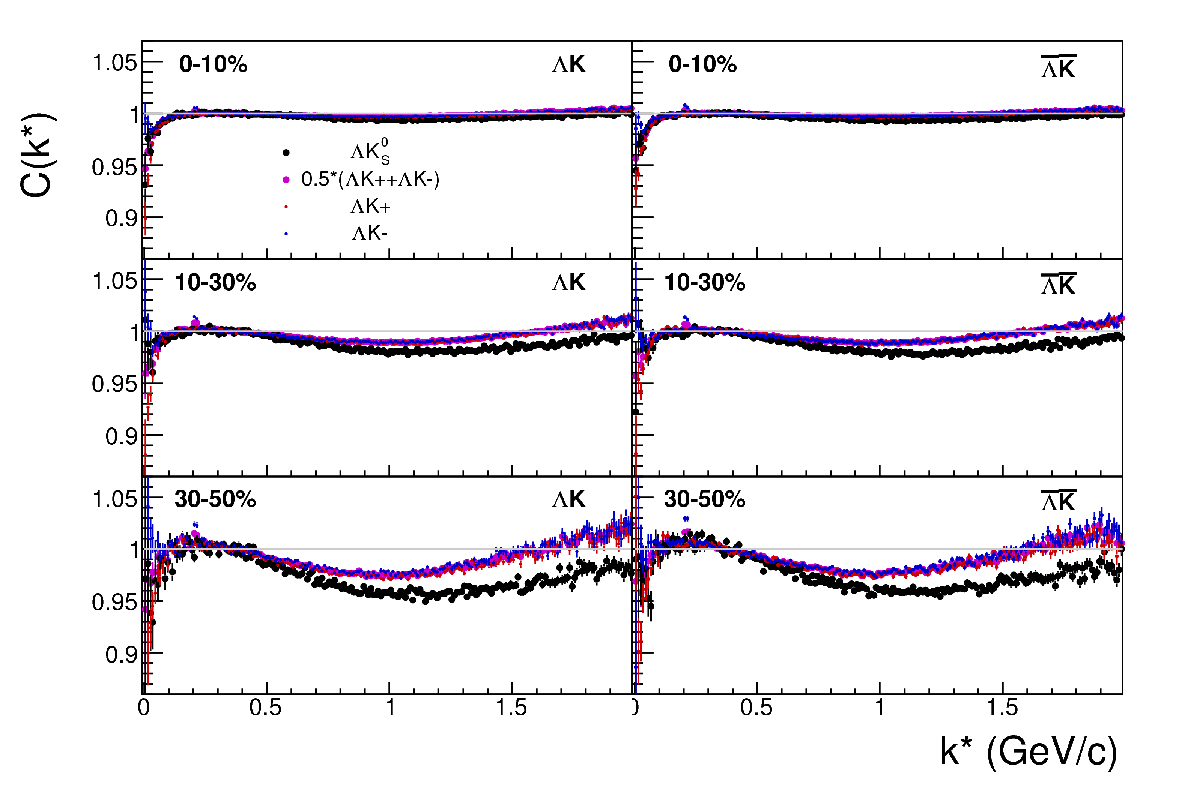
\includegraphics[width=\textwidth]{5_Fitting/Figures/CompareLamKchAvgToLamK0_wIndivKch_0010_1030_3050.pdf}
  \caption[Compare Backgrounds]{Compare backgrounds}
  \label{fig:CompareAllBgds}
\end{figure}

It is suggested that this background effect is due primarily to particle collimation associated with elliptic flow \cite{Kisiel:2017}.  More specifically, these backgrounds result from mixing events with unlike event-plane angles ($\Psi_{\textrm{EP}}$).  As explained in \cite{Kisiel:2017}, when elliptic flow is present, all particles are more likely to be emitted in a specific direction (in-plane), as opposed to a perpendicular direction.  Therefore, the difference in momenta for pairs of particles tends to be smaller, compared to the case of no flow.  In the case of mixed-event pairs, the two events used do not share an event-plane, and therefore this is no collimation effect in the pairs from flow.  As a result, pairs with larger momentum are more likely when mixed-events are used, and the correlation function will be observed below unity.  In general, a dip below unity, at a given $k^{*}$, means it is more probable to find a pair at that $k^{*}$ when the daughters are taken from mixed-events, as compared to when they are taken from the same event.

This same reasoning suggests that the background should lead to an enhancement at low-$k^{*}$.  The enhancement at high-$k^{*}$ ($k^{*} \gtrsim$ 1.5 GeV/$c$) does not result from the collective flow of the system.  We are not certain was causes this enhancement, but typical suspects are jet-like correlations and resonance decays.

We can split our correlation functions into three main regions.  First, the low-$k^{*}$ region ($k^{*} \lesssim 0.3$ GeV/$c$) contains the femtoscopic correlations, as well as a likely enhancement from the background.  The intermediate-$k^{*}$ region (0.3 $\lesssim k^{*} \gtrsim$ 1.5 GeV/$c$) contains a suppression from the background.  Finally, the high-$k^{*}$ region ($k^{*} \gtrsim$ 1.5 GeV/$c$) contains an enhancement with unknown origin.


\begin{figure}[h!]
  \centering
  %%----start of first subfigure---  
  \subfloat[\LamKchP]{
    \label{fig:BgdswTHERM:a}
    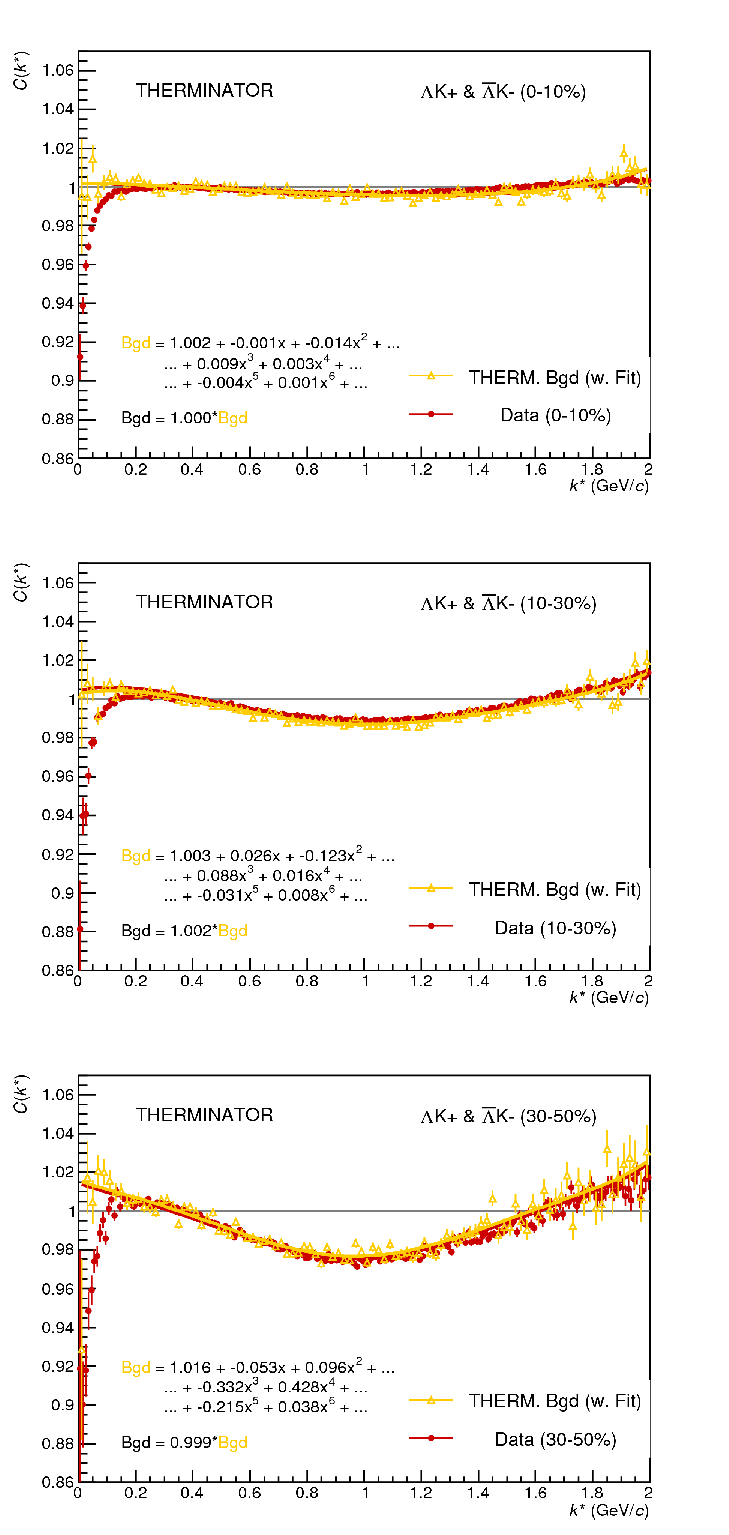
\includegraphics[width=0.33\textwidth]{5_Fitting/Figures/BgdwFitOnly_RandomEPs_NumWeight1_PrimaryOnly_LamKchPwConj_0010_1030_3050.pdf}}
  %%----start of second subfigure---
  \subfloat[\LamKchM]{
    \label{fig:BgdswTHERM:b}
    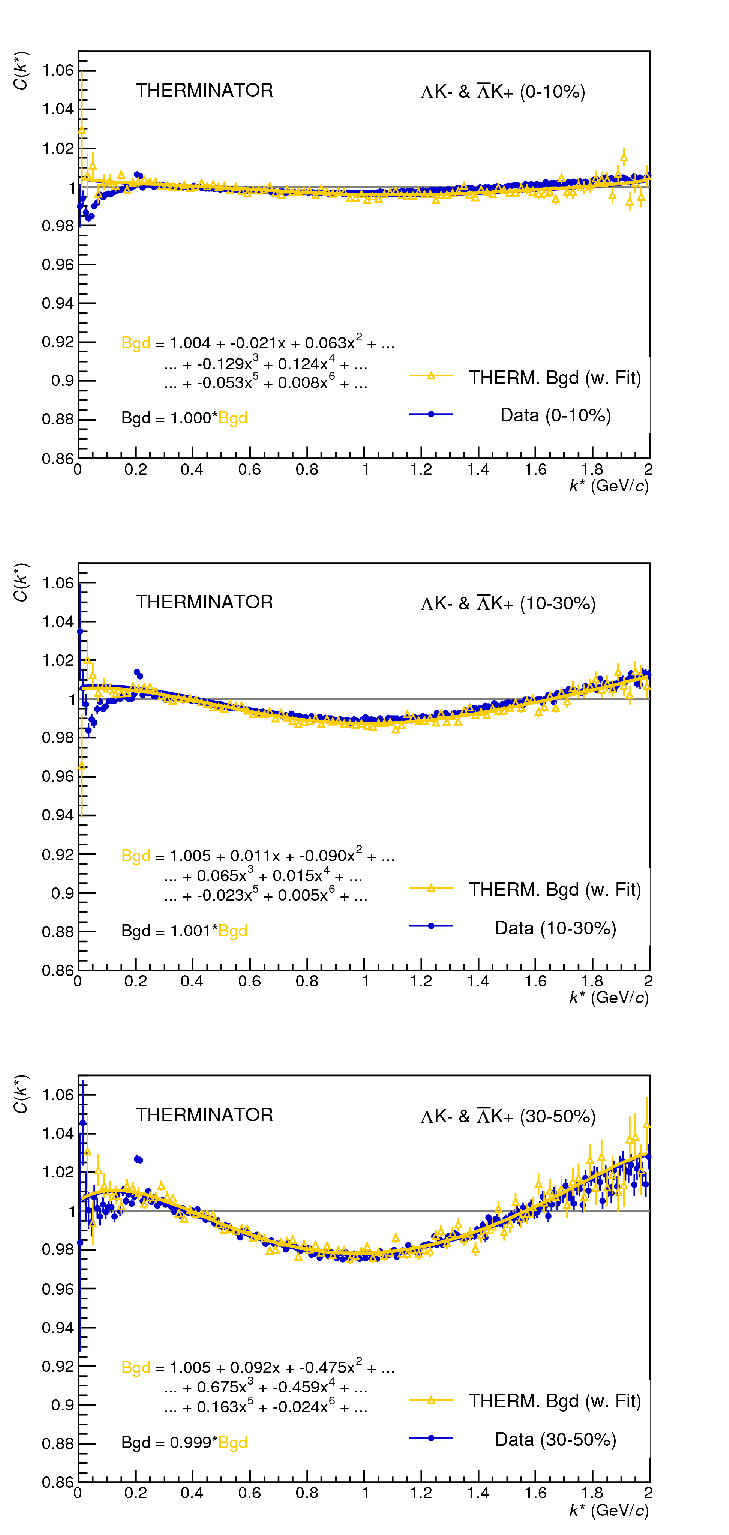
\includegraphics[width=0.33\textwidth]{5_Fitting/Figures/BgdwFitOnly_RandomEPs_NumWeight1_PrimaryOnly_LamKchMwConj_0010_1030_3050.pdf}}
  %%----start of third subfigure---
  \subfloat[\LamKs]{
    \label{fig:BgdswTHERM:c}
    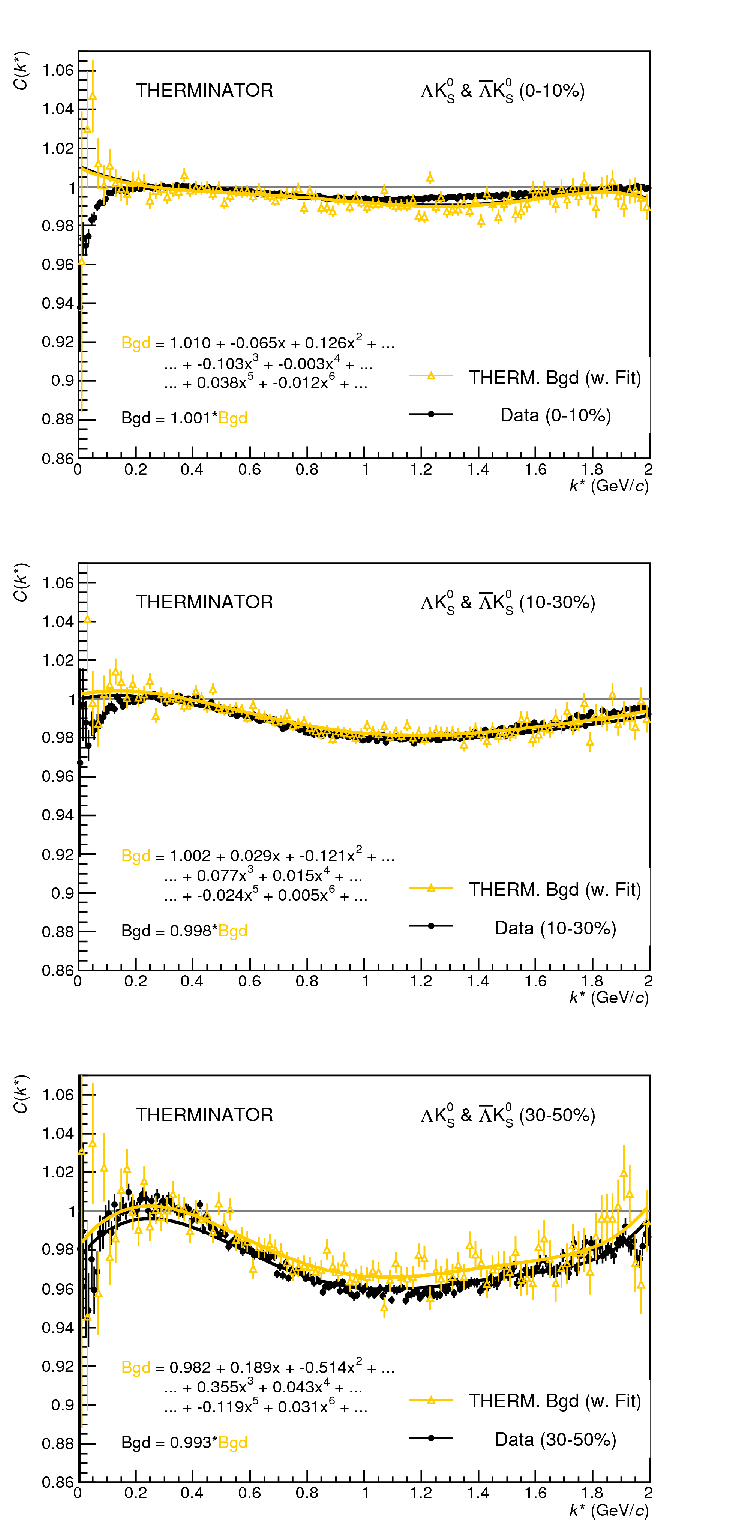
\includegraphics[width=0.33\textwidth]{5_Fitting/Figures/BgdwFitOnly_RandomEPs_NumWeight1_PrimaryOnly_LamK0wConj_0010_1030_3050.pdf}}    
  %%----overall caption----
  \caption[Backgrounds with THERMINATOR]{Backgrounds with THERMINATOR}
  \label{fig:BgdswTHERM}
\end{figure}


\begin{figure}[h]
  \centering
  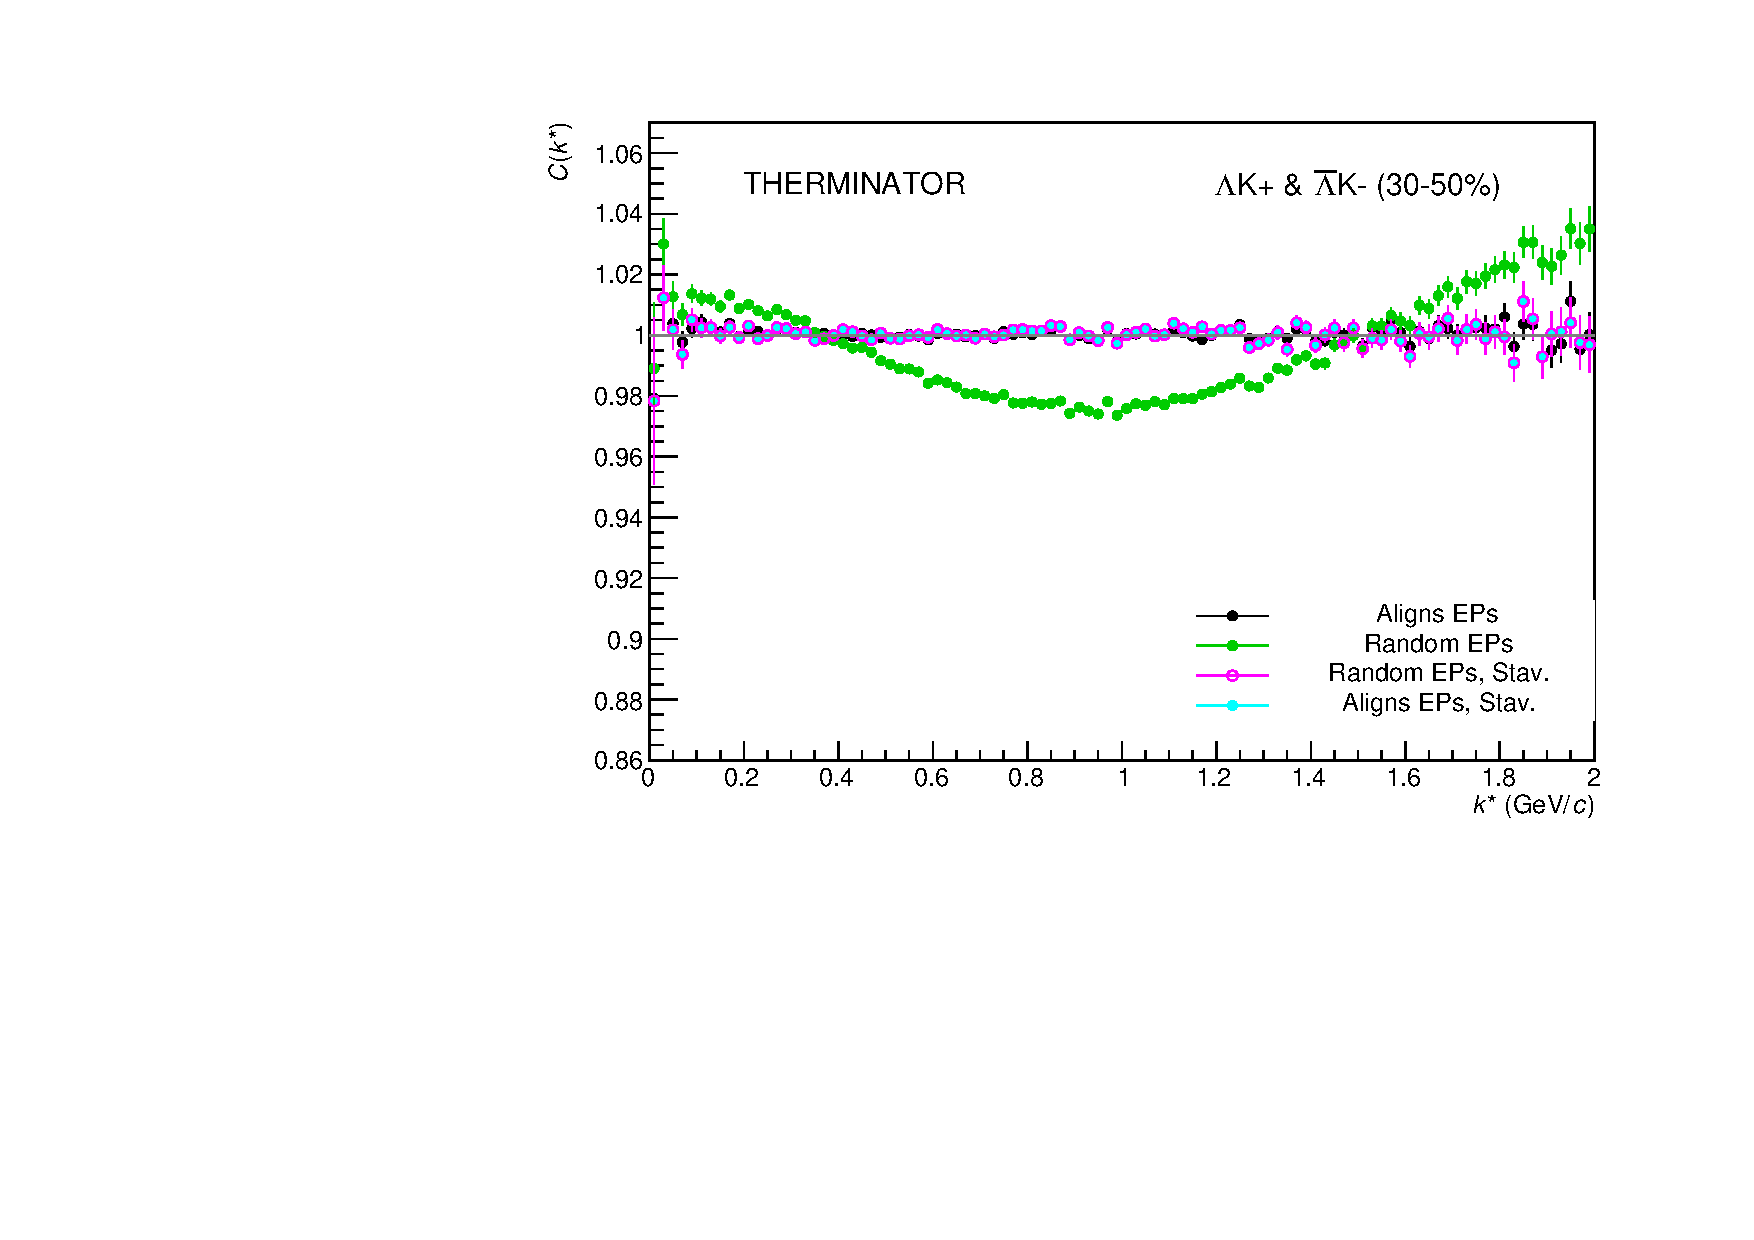
\includegraphics[width=\textwidth]{5_Fitting/Figures/CompareBackgroundReductionMethods_Full_LamKchPwConj_3050_NumWeight1.pdf}
  \caption[Background reduction methods with THERMINATOR]{Background reduction methods with THERMINATOR}
  \label{fig:BgdRedMethodsTHERM}
\end{figure}



\begin{figure}[h]
  \centering
  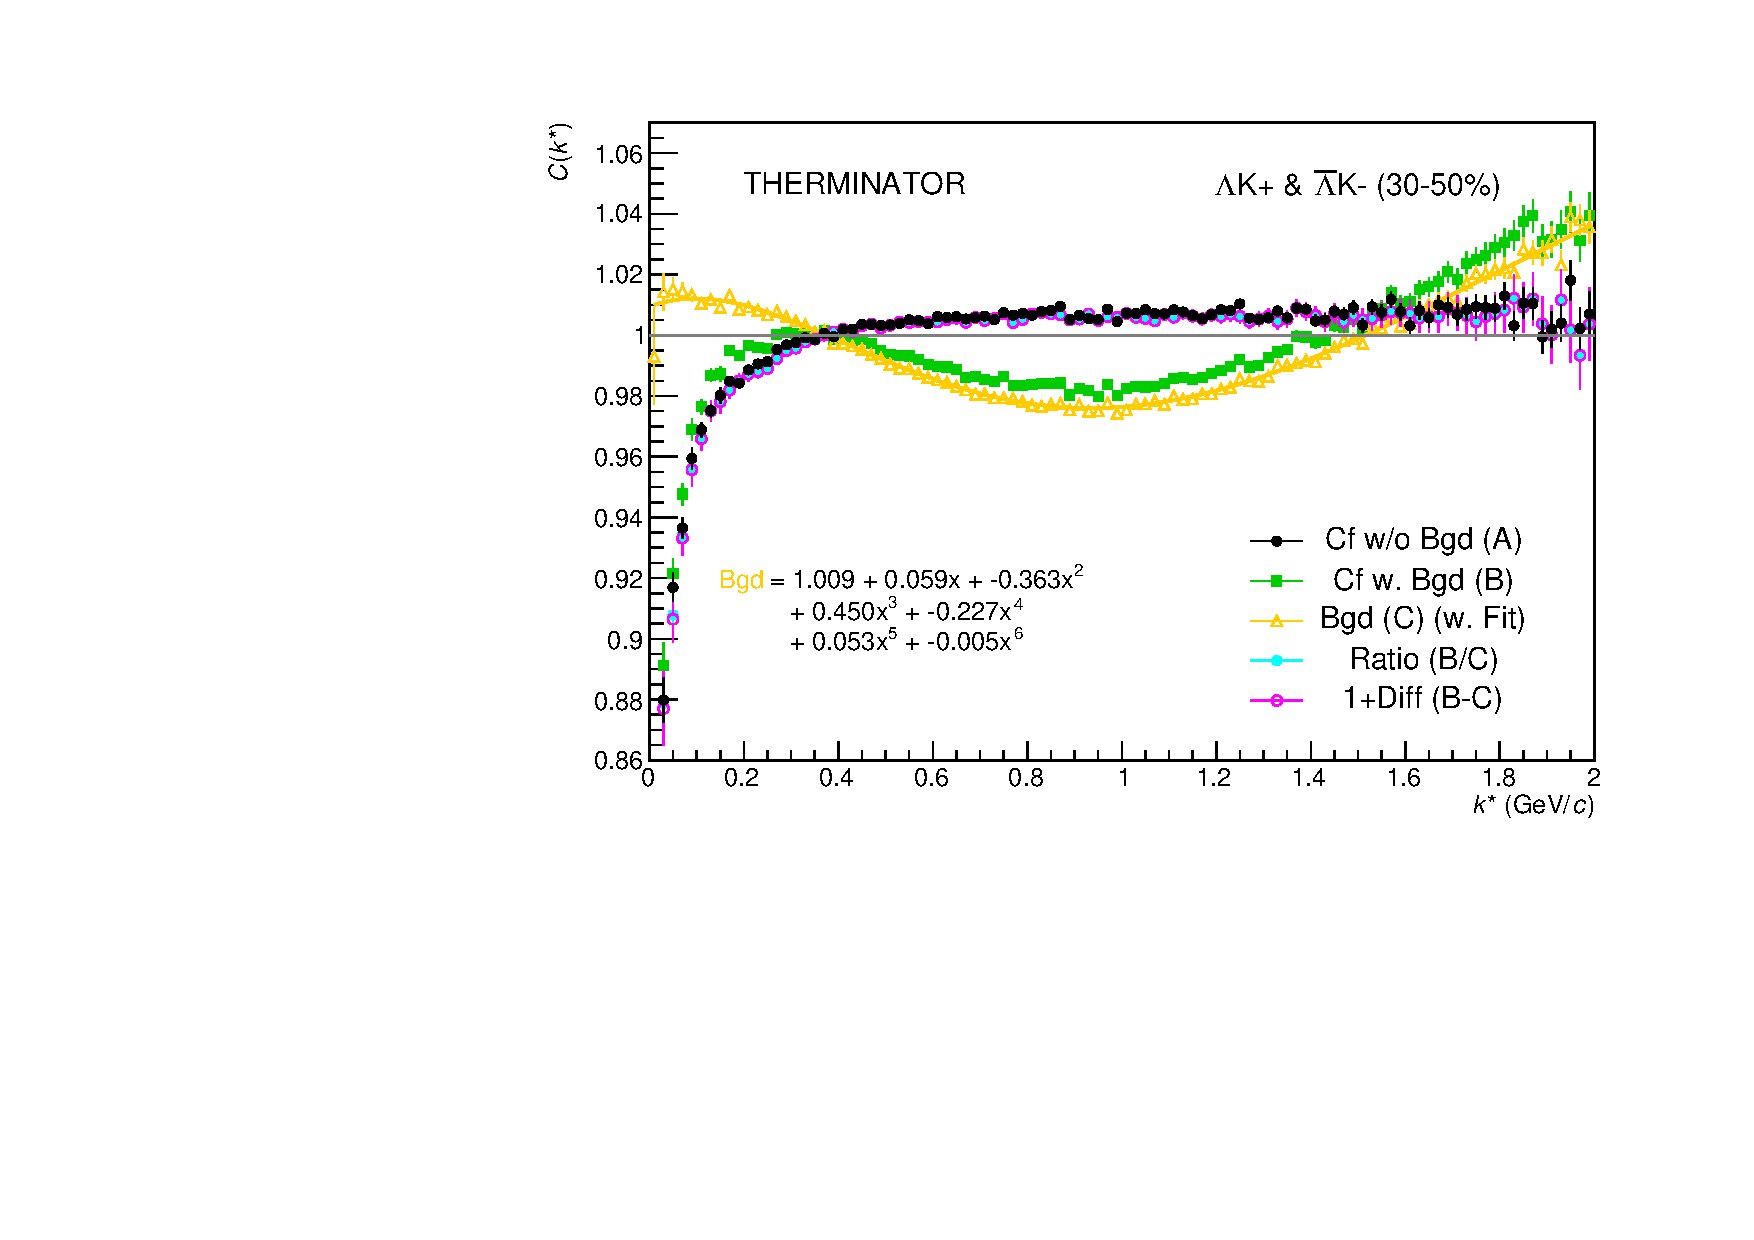
\includegraphics[width=\textwidth]{5_Fitting/Figures/CompareBgds_Full_LamKchPwConj_3050.pdf}
  \caption[Correlation with background decomposition (THERM)]{Correlation with background decomposition with THERMINATOR}
  \label{fig:THERMCfBgdDecomposition}
\end{figure}




\end{document}